\documentclass[10pt, border=10pt]{standalone}
\input{../../tikzpic_packages.tex}

\def\pneumaticcolor{blue!20}

\begin{document}

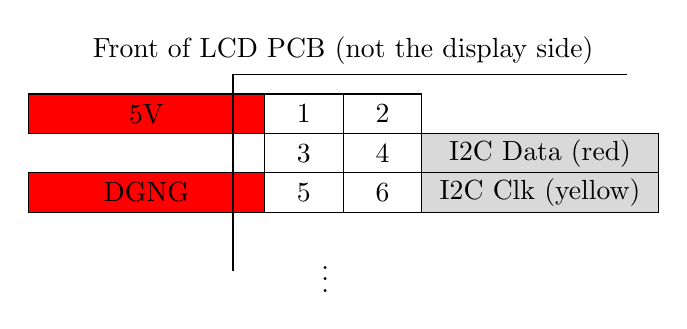
\begin{tikzpicture}[
gpio/.style={fill=green},
ain/.style={fill=blue!40},
pwm/.style={fill=purple!70},
pwr/.style={fill=red},
i2c/.style={fill=gray!30},
pins/.style={midway},
fun/.style={midway, black},
stats/.style={draw=none}
]

\def\w{3}
\def\ws{1}
\def\h{.5}


%%% P8
\path (\w+\w+\w,0) coordinate(O)++(\ws,\h)node[above, scale=1]{Front of LCD PCB (not the display side)};
\foreach \i in {1,...,6}{
	\pgfmathsetmacro{\shift}{mod(\i-1,2)*\ws}
	\pgfmathsetmacro{\y}{(\i-\shift)*.5*\h}
	\ifodd\i
		\path (O)++(\shift,-\y)coordinate(\i);
	\else
		\path (O)++(\shift+\ws,-\y)coordinate(\i); \fi
	\draw (O)++(\shift,-\y)rectangle++(\ws,\h)node[pins]{\i};
}

\foreach \pin/\fun/\txt in {
	1/pwr/5V,
	4/i2c/I2C Data (red),
	6/i2c/I2C Clk (yellow),
	5/pwr/DGNG
	}{
	\ifodd\pin
		\draw[\fun](\pin)rectangle++(-\w,\h)node[fun]{\txt};
	\else
		\draw[\fun](\pin)rectangle++(\w,\h)node[fun]{\txt}; \fi
	}

%
%%%% Legend
%\path (\w+\w+\w+\ws+\ws+.2,-\w) coordinate(O)node[above right]{Legend:};
%\foreach[count=\i] \cat in {pwr, i2c}{
%	\pgfmathsetmacro{\y}{\i*\h}
%	\draw[\cat](O)++(0,-\y)rectangle++(\w-.2,\h)node[fun]{\cat};
%}

\draw (O)++(-.4,-2) node[right=1cm]{$\vdots$}--++(0,2.5)--++(5,0);


\end{tikzpicture}
\end{document}